\documentclass{article}
\usepackage{pythonhighlight}
\usepackage{graphicx}
\usepackage{ctex}
\usepackage[left=3cm,top=3cm,right=3cm]{geometry}
\usepackage{hyperref}
% TITLE PAGE CONTENT %%%%%%%%%%%%%%%%%%%%%%%%
%%%%%%%%%%%%%%%%%%%%%%%%%%%%%%%%%%%%%%%%%%%%%
\newcommand{\labno}{09}
\newcommand{\labtitle}{EE208 Hadoop Streaming}
\newcommand{\authorname}{周李韬}
\newcommand{\studentno}{518030910407}
\newcommand{\classno}{F1803016}
% END TITLE PAGE CONTENT %%%%%%%%%%%%%%%%%%%%


\begin{document}

\begin{center}
{\LARGE \textsc{Laboratory No. \labno:} \\ \vspace{4pt}}
{\Large \textsc{\labtitle} \\ \vspace{4pt}} 
\rule[13pt]{\textwidth}{1pt} \\ \vspace{15pt}
{\large By: \authorname \\ \vspace{10pt}
No. \studentno \\ \vspace{10pt}
SJTU \classno \\ \vspace{10pt}
\today \vspace{20pt}}
\end{center}



\section{实验准备}

\subsection{实验环境}
\begin{itemize}
\item\textbf{Environment} Ubuntu 16.04 (on Virtual Machine)
\item\textbf{Tools} Hadoop 2.7.3, openjdk-8-jdk
\end{itemize}

\subsection{实验目的}

本实验中,我们需要借助Hadoop中的Map-Reduce模型,实现分布式地计算文章中单词平均长度,计算一张图中的PageRank。

\subsection{实验原理}

Map-Reduce的原理在上一次实验中已阐述。简单来说,Map对输入数据进行运算后,会产生一系列中间变量,随后Reduce函数对中间变量进行运算,得到输出结果。其中,Map和Reduce过程需要能够实现分布式运算。在Hadoop的MapReduce模型中,在Map和Reduce之间,会有一次对数据的排序过程,利用这一功能,Map结果将会按照数据的Key排序,从而使下一步Reduce提供帮助。

\paragraph{计算单词平均长度}

我们可以采用和WordCount Example类似的思想解决计算单词平均长度的问题。对读入的每个单词,我们将其通过Map函数产生(首字母,单词长度,单词个数(初始值为1))的记录,在Reduce函数中,对相同首字母的记录做合并操作,将单词长度、单词个数进行累加,最后输出单词长度和单词个数之商,就得到了所有首字母开头的单词的平均长度分布。


\paragraph{计算PageRank}
本实验中,我们通过迭代的方式计算图的PageRank。在一次迭代中,我们通过以下公式计算一个点的PageRank。
$$ PageRank(v) = \sum_{(u,v)\in \mathbf{G}} {\frac{PageRank(u)}{OutDegree(u)}}$$

数学中可以证明,在对所有节点进行该运算后,一次迭代运算的结果中所有节点的PageRank之和仍为1,且在连通性较好的情况下中,多次迭代能够收敛到页面真实的PageRank值。

在分布式实现方面,我们假设图是以邻接表的形式存储在文本文件中的,由于图的结构在运算过程中只会被读取,不会被修改,因此我们考虑在实验中将图作为一组静态数据,在输入时图结构会被Map函数读入参与运算,在Reduce过程中,参与运算后就会被消去。在下一次迭代时,再重新通过Map函数读取静态的图结构邻接表参与PageRank的运算。

与静态的邻接表相对的是存储每个节点PageRank的PageRank向量。我们通过一个(节点,PageRank)的列表存储该数据。在Map过程中,我们对每一个点,可以通过图邻接表读取它的所有出点,通过PageRank向量读取节点的PageRank值,我们将PageRank除以该节点邻接表的长度,使得该节点的PageRank平均分配给它的每一个出点。我们将出点和由当前节点贡献的rank值作为中间值返回。

由于在执行Reduce之前,Hadoop会对各中间值按照KEY进行排序,因此相同KEY的(节点,subRank)记录会被相邻排列。不难通过Reduce过程将相同节点的Rank值相加合并。最终的输出就是经过一次迭代后的PageRank向量。

在迭代的实现方面,我们使用bash,循环调用Hadoop中的Map-Reduce命令,每一次迭代的输出就是下一次迭代的输入,直到达到一定的迭代次数退出,输出各节点最终的PageRank值。

\section{实验步骤}

\subsection{计算单词平均长度}
\subsubsection{Mapper}
在Mapper部分,我们需要读入文本文件的每一行,拆分单词,输出其首字母、长度。代码如下所示:
\begin{python}
#!/usr/bin/env python

import sys

for line in sys.stdin:        # 遍历输入的每一行文件
    line = line.strip()       # 去除首尾空格
    words = line.split()      # 分割单词
    for word in words:
        print '%s\t%s\t%s' % (word[0],len(word),1)
                              # 输出单词首字母,长度,统计个数
\end{python}

\subsubsection{Reducer}
在Reducer部分,根据Map后的排序结果,相同首字母的单词将会排列在一起,因此我们可以连续地读取Mapper产生的数据,并且在累加统计完毕后,换到另一个不同首字母时,输出统计的平均值结果。代码如下所示:
\begin{python}
#!/usr/bin/env python

import sys

current_word = None
current_count = 0
current_length = 0
word = None
for line in sys.stdin:
    line = line.strip()
    word,length,count = line.split('\t',2)  # 读取Mapper结果
    try:
        count = int(count)
        length = int(length)
    except ValueError:
        continue
    if current_word == word:      # 对关键词相同的记录,累加
        current_count += count
        current_length += length
    else:                         # 对关键词不同的记录
        if current_word:          # 输出上一条记录的均值
            print current_word, float(current_length)/current_count
        current_count = count     # 开始新的统计
        current_word = word
        current_length = length

if current_word== word:           # 输出最后一类记录的统计结果
    print current_word, float(current_length)/current_count
\end{python}

\subsubsection{Chainer}
尽管本实验中并没有用到多步迭代的功能,但为了方便实现封装,我们提供了一个bash文件执行Hadoop的一系列操作。包括清空上一次的tempoutput文件,将当前系统目录下的txt文件拷贝到Hadoop文件系统中,调用mapper、reducer完成运算等,bash代码已附在辅助材料中。


\subsubsection{实验结果}
我们在pg4300.txt文件上运行MapReduce函数,运行过程如图\ref{wcrun}所示。我们得到的文章中平均单词长度的统计结果如图\ref{wcres1}、\ref{wcres2}所示。
\begin{figure}[htbp]
\centering
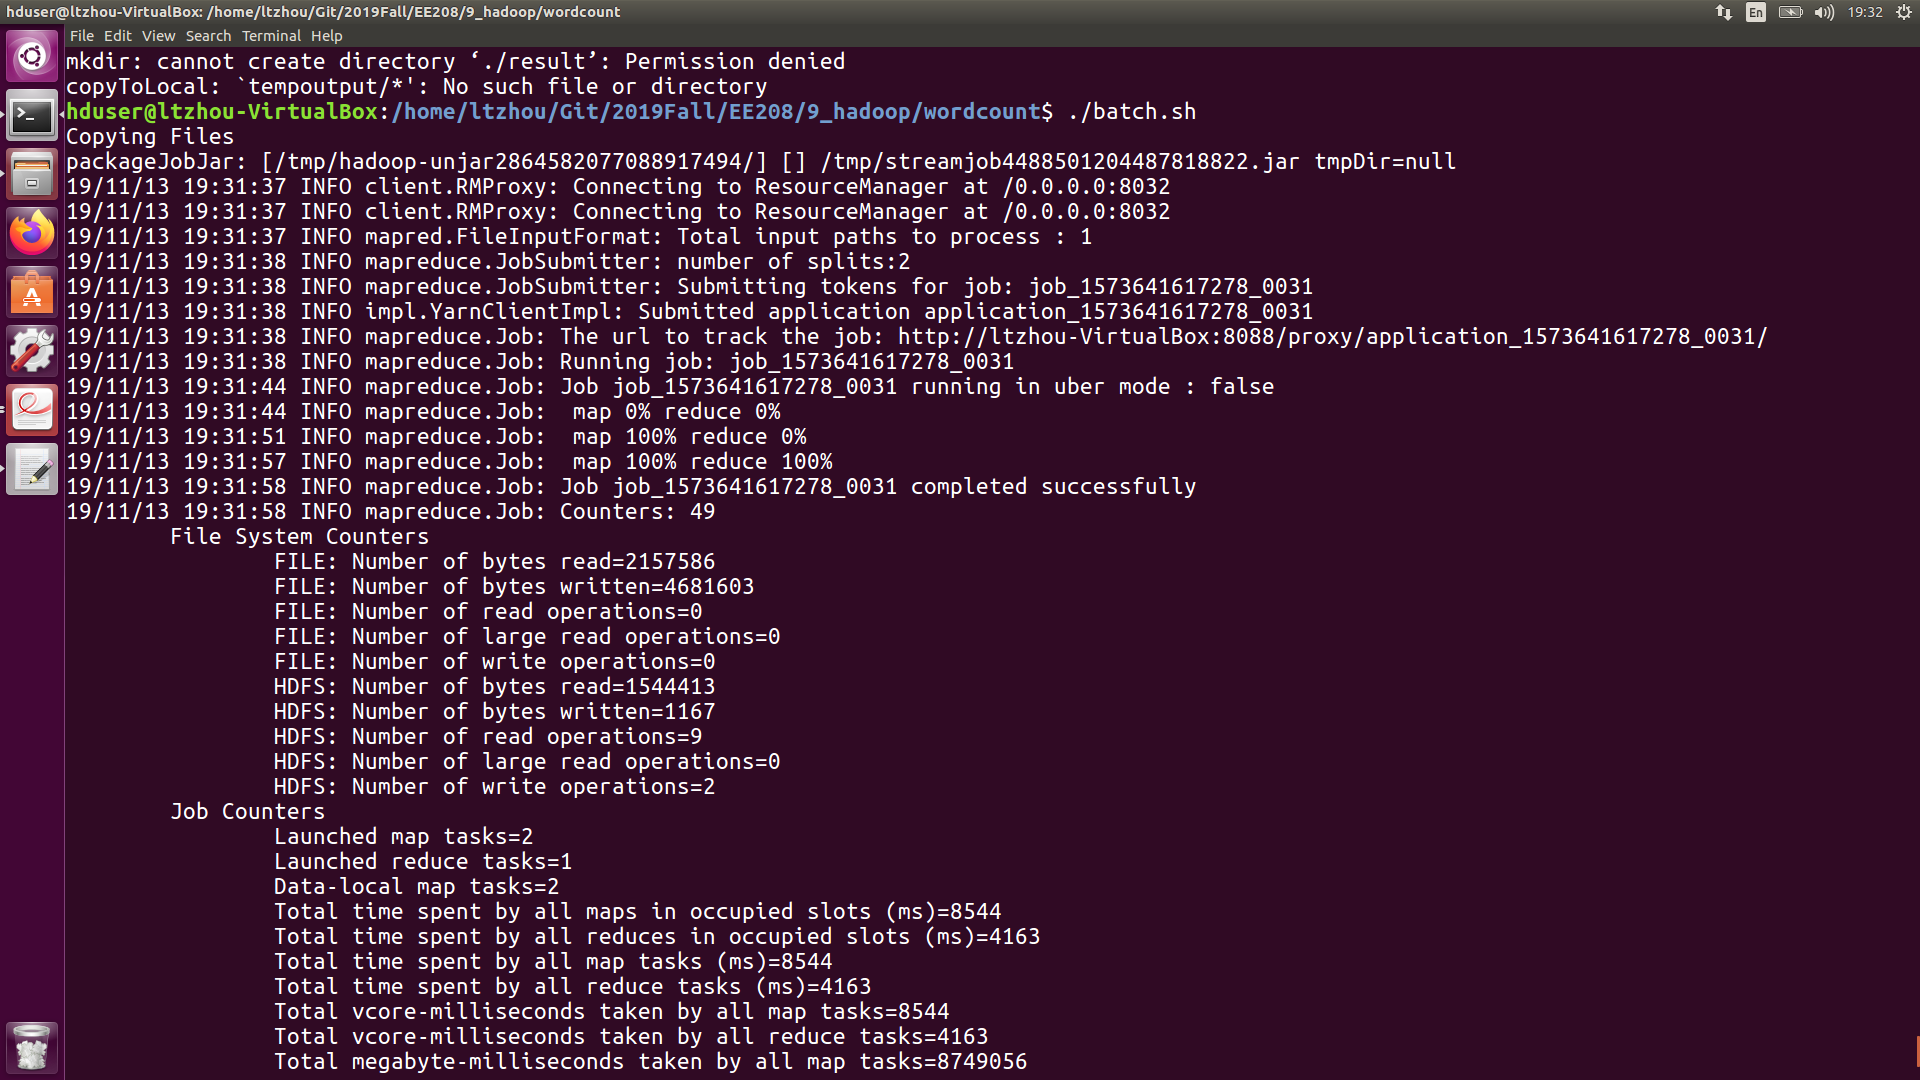
\includegraphics[width=7.5cm]{img/wc_running_head.png}
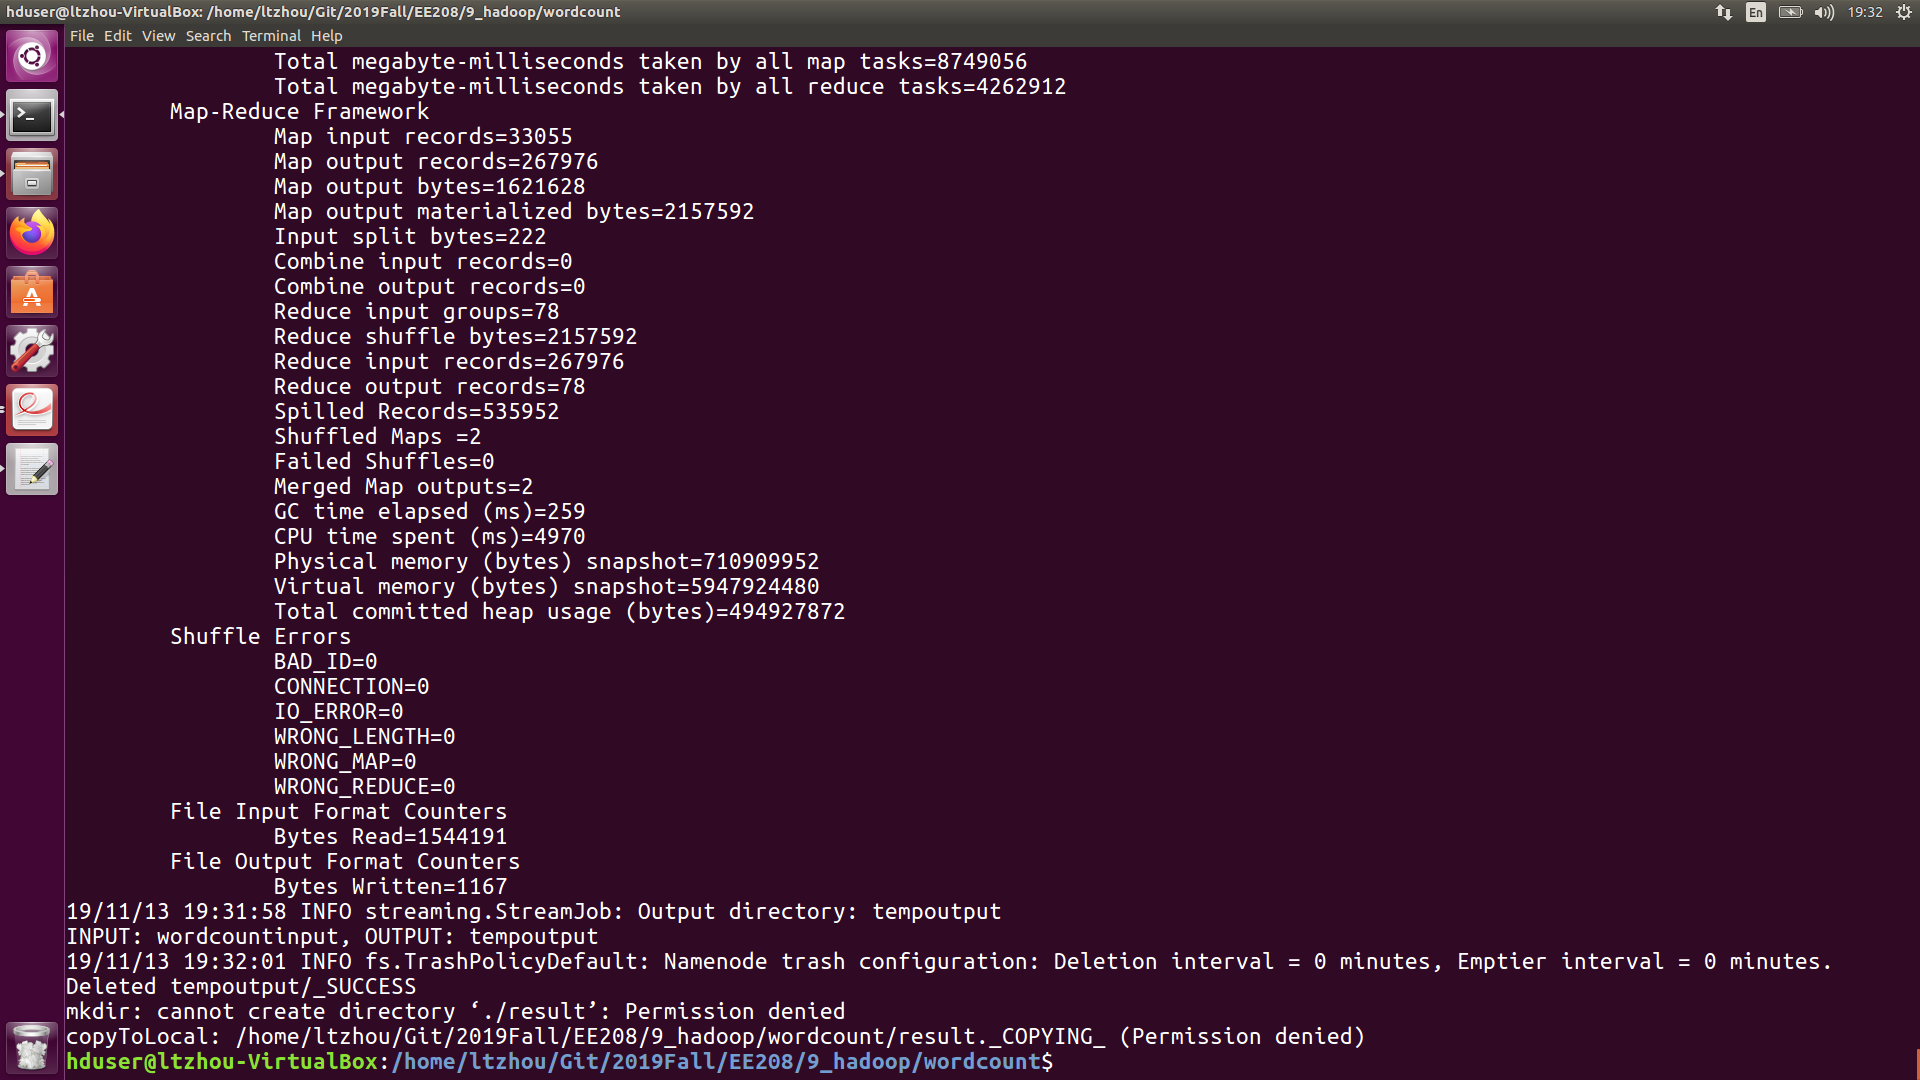
\includegraphics[width=7.5cm]{img/wc_running_end.png}
\caption{单词长度统计程序运行示例}
\label{wcrun}
\end{figure}

\begin{figure}[htbp]
\centering
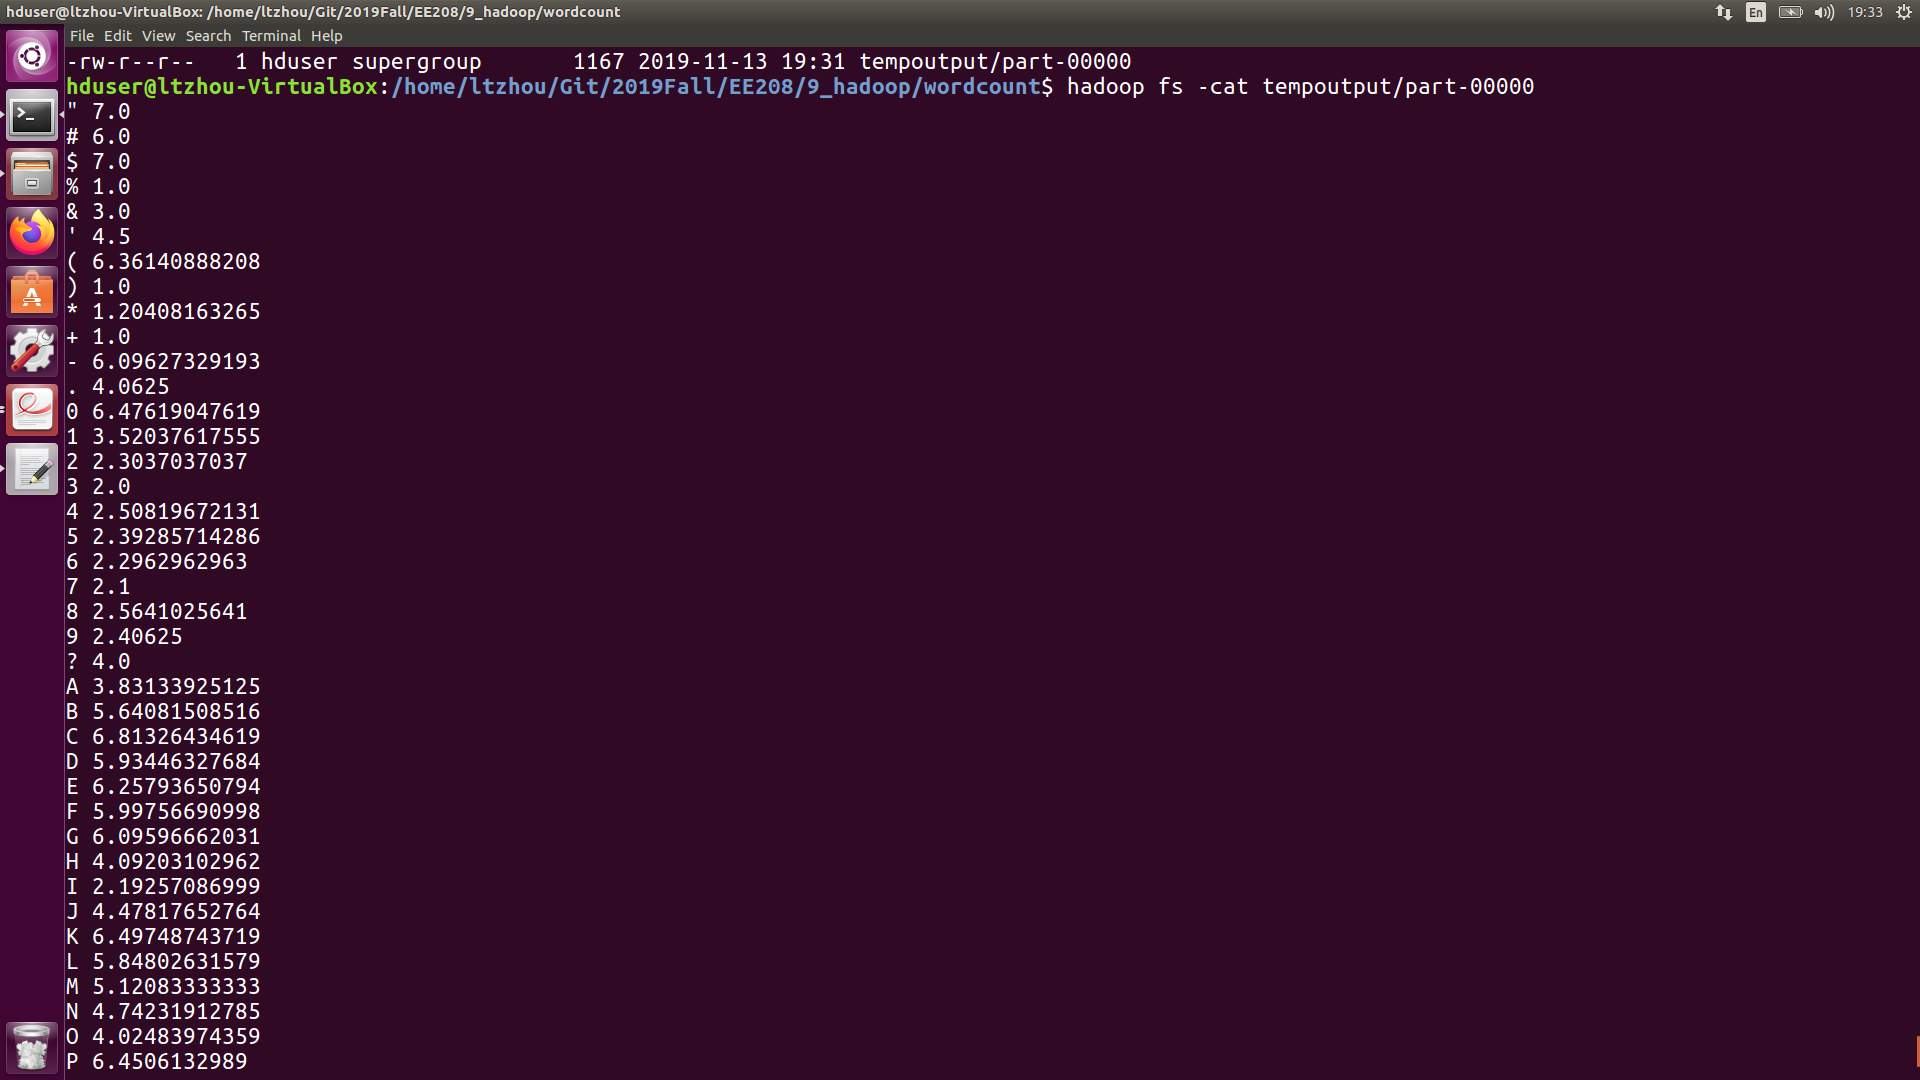
\includegraphics[width=14.5cm]{img/wc_output1.png}
\caption{pg4300单词平均长度统计结果}
\label{wcres1}
\end{figure}
\begin{figure}[htbp]
\centering
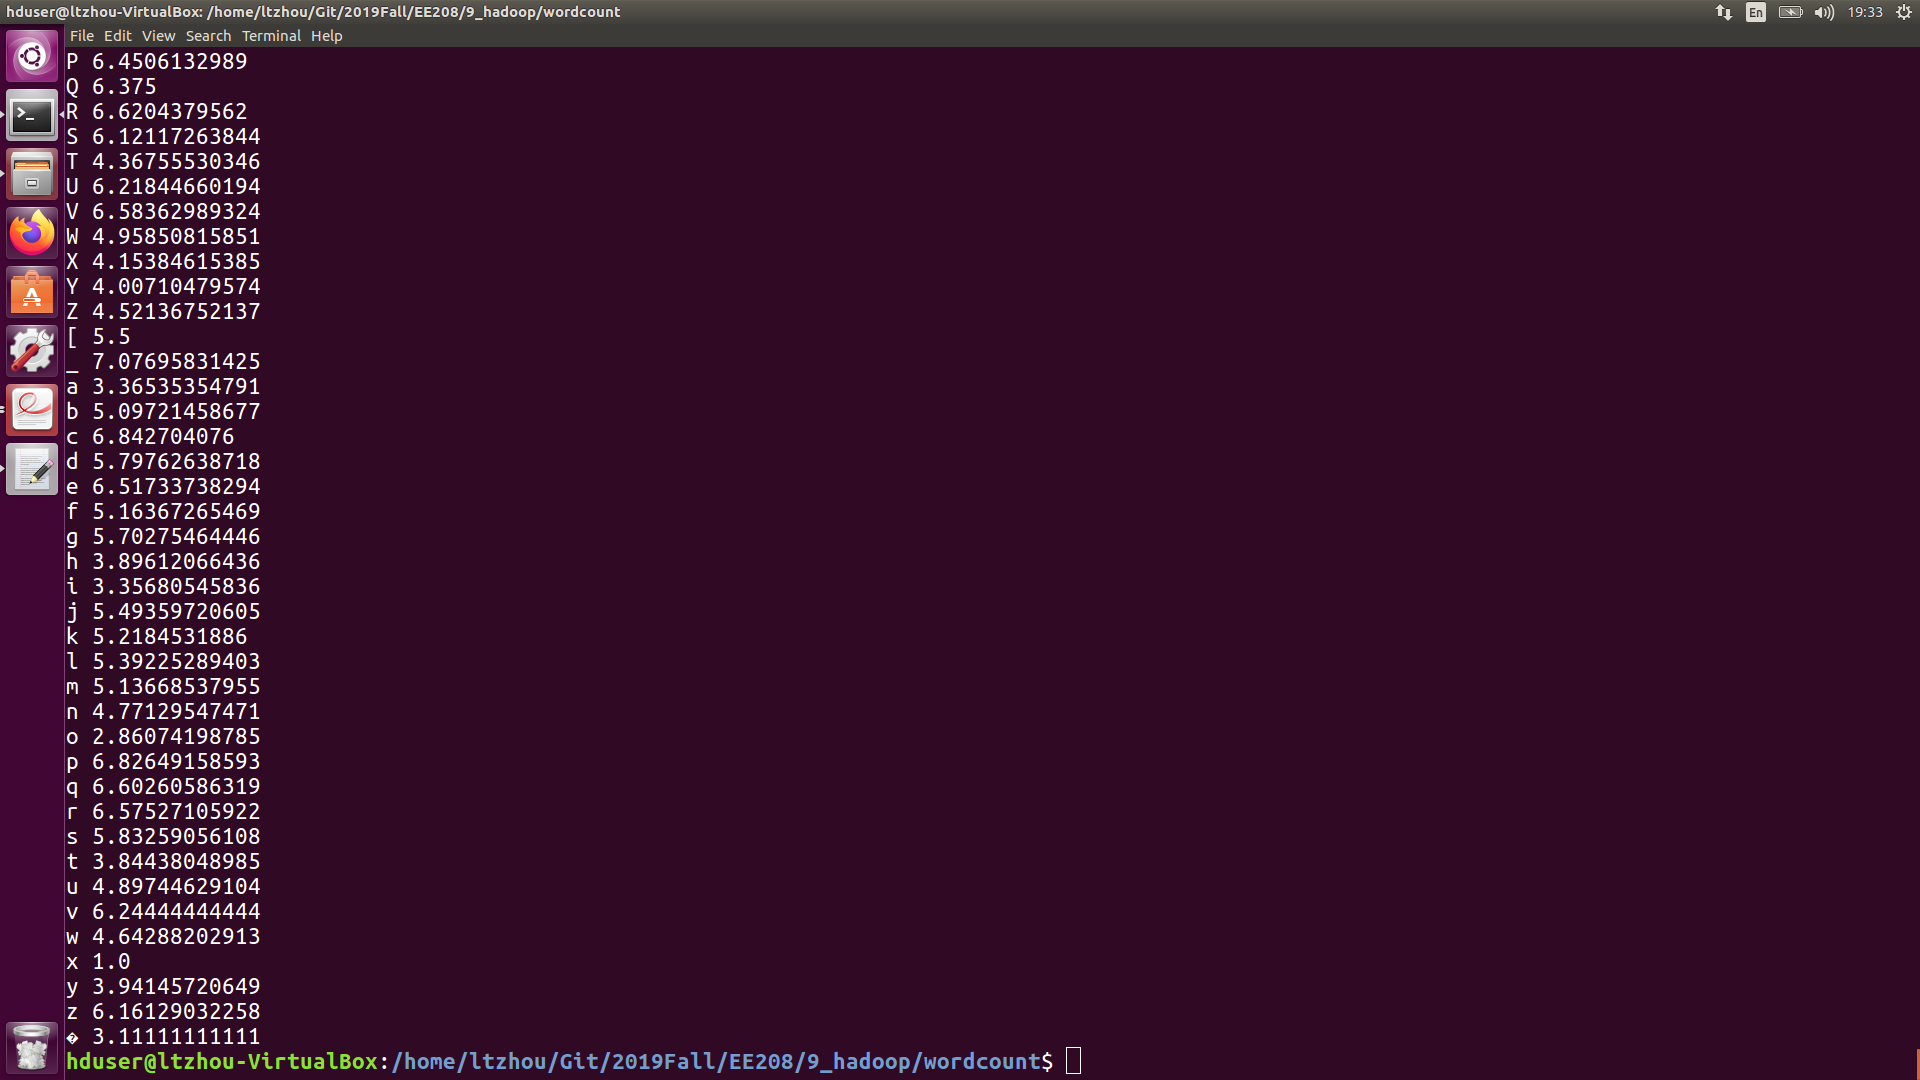
\includegraphics[width=14.5cm]{img/wc_output2.png}
\caption{pg4300单词平均长度统计结果}
\label{wcres2}
\end{figure}

该实验表明,尽管文章的次数很长,但分布式的运算能够有效利用计算机设备的性能,在较短的时间内完成单词词长的统计。

\subsection{计算图的PageRank}
\subsubsection{Mapper}
根据上文的实验原理所述,在Mapper部分,我们会读入两条数据,一个节点的邻接表和它的当前PageRank值,Map的返回结果是一个(出点,该出点分到的PageRank值)二元对。Python代码如下所示。按照排序关系,PageRank值的记录会先于邻接表记录出现,因此在Map的循环中,当一条记录的节点发生改变时,说明读到了PageRank值,没有发生改变时,说明读到了邻接表。根据这一关系,我们可以建立对应的分支程序。
\begin{python}
# map for subrank (src, rank);(src, dsts) -> (dst, subrank)
current_src = None
current_dst = None
current_degree = 0
current_rank = 0

for line in sys.stdin:
    line = line.strip()
    if len(line) > 0:
        seg = line.split()
        src = seg[0]
        if (src != current_src):         # 读取节点的PageRank值
            current_src = src
            current_rank = float(seg[1])
        else:                            # 读取节点的邻接表
            if (len(seg)>1):
                current_dst = seg[1:]
                current_degree = len(current_dst)  # 计算节点的出度
                subrank = current_rank/current_degree
                for dst in current_dst:  # 将节点PageRank平均分给它的出点,产生Map中间值。
                    print '%s\t%s' % (dst,subrank)
\end{python}

\subsubsection{Reducer}
在Reducer中,我们只需要将Mapper结果中,相同的节点从各处分到的PageRank值相加即可,由于Mapper结果已经被排序,我们可以通过与WordCount Example中类似的结构实现,此处不再详述。需要注意的一点是,由于PageRank计算的结果是浮点数,因此我们在输入输出时,不仅要关注类型的转换,还要注意不应让浮点数小数位数过长,否则会极大拖慢Hadoop的运行速度,甚至报Runtime Error错误。因此,为方便起见,本实验中计算的精度统一取两位小数,输出代码如下所示,
\begin{python}
if (src != current_src):  # 读取新的节点记录
    if (current_src):     # 输出上一个节点的PageRank值
        print '%s %.2f' % (current_src, current_rank)  # 输出浮点数
    current_src = src     # 开始新的一轮统计
    current_rank = float(seg[1])  # 读入浮点数
\end{python}

\subsubsection{Chainer}
我们注意到,在本实验中,Mapper的输入不止有PageRank向量,还有图的邻接表结构,这两组数据分别存于不同的文件中,而Mapper要求PageRank和图邻接表需要做到节点的一一对应,相互间隔排列。因此仅有上述所说的Mapper和Reducer是不够的,我们在将两组数据输入Mapper之前,还要对其进行排序。为此我们写了下面这样一个简单的Mapper,相当于调用了一次Map-Reduce函数,但在这一轮Map-Reduce中,Mapper和Reducer都没有做任何事情,我们只是利用了Hadoop封装的排序功能。
\begin{python}
import sys

# map graph
for line in sys.stdin:
    line = line.strip()
    print line
\end{python}

在经过排序后,调用上述的RankMapper和Reducer就能够实现为每一个节点重新分配PageRank了。PageRank的计算是一个迭代的过程,为此我们需要通过Bash反复调用Map-Reduce函数,同时我们还要有效管理每次调用的输入和输出,使得前一次迭代的输出是后一次迭代的输入,这可以通过在bash中创建文件名变量的方式实现。bash代码已附在辅助材料中。

\subsubsection{实验结果}



我们对一个简单图结构运行迭代程序计算PageRank,迭代10次,样例数据如下,运行过程如图\ref{prrun}所示。
\begin{python}
# Graph Structure
src | dst      | Initial PageRank
-----------------------------------
 A  | B C D    | 0.25
 C  | A        | 0.25
 B  | C        | 0.25
 D  | C B      | 0.25
\end{python}

\begin{figure}[htbp]
\centering
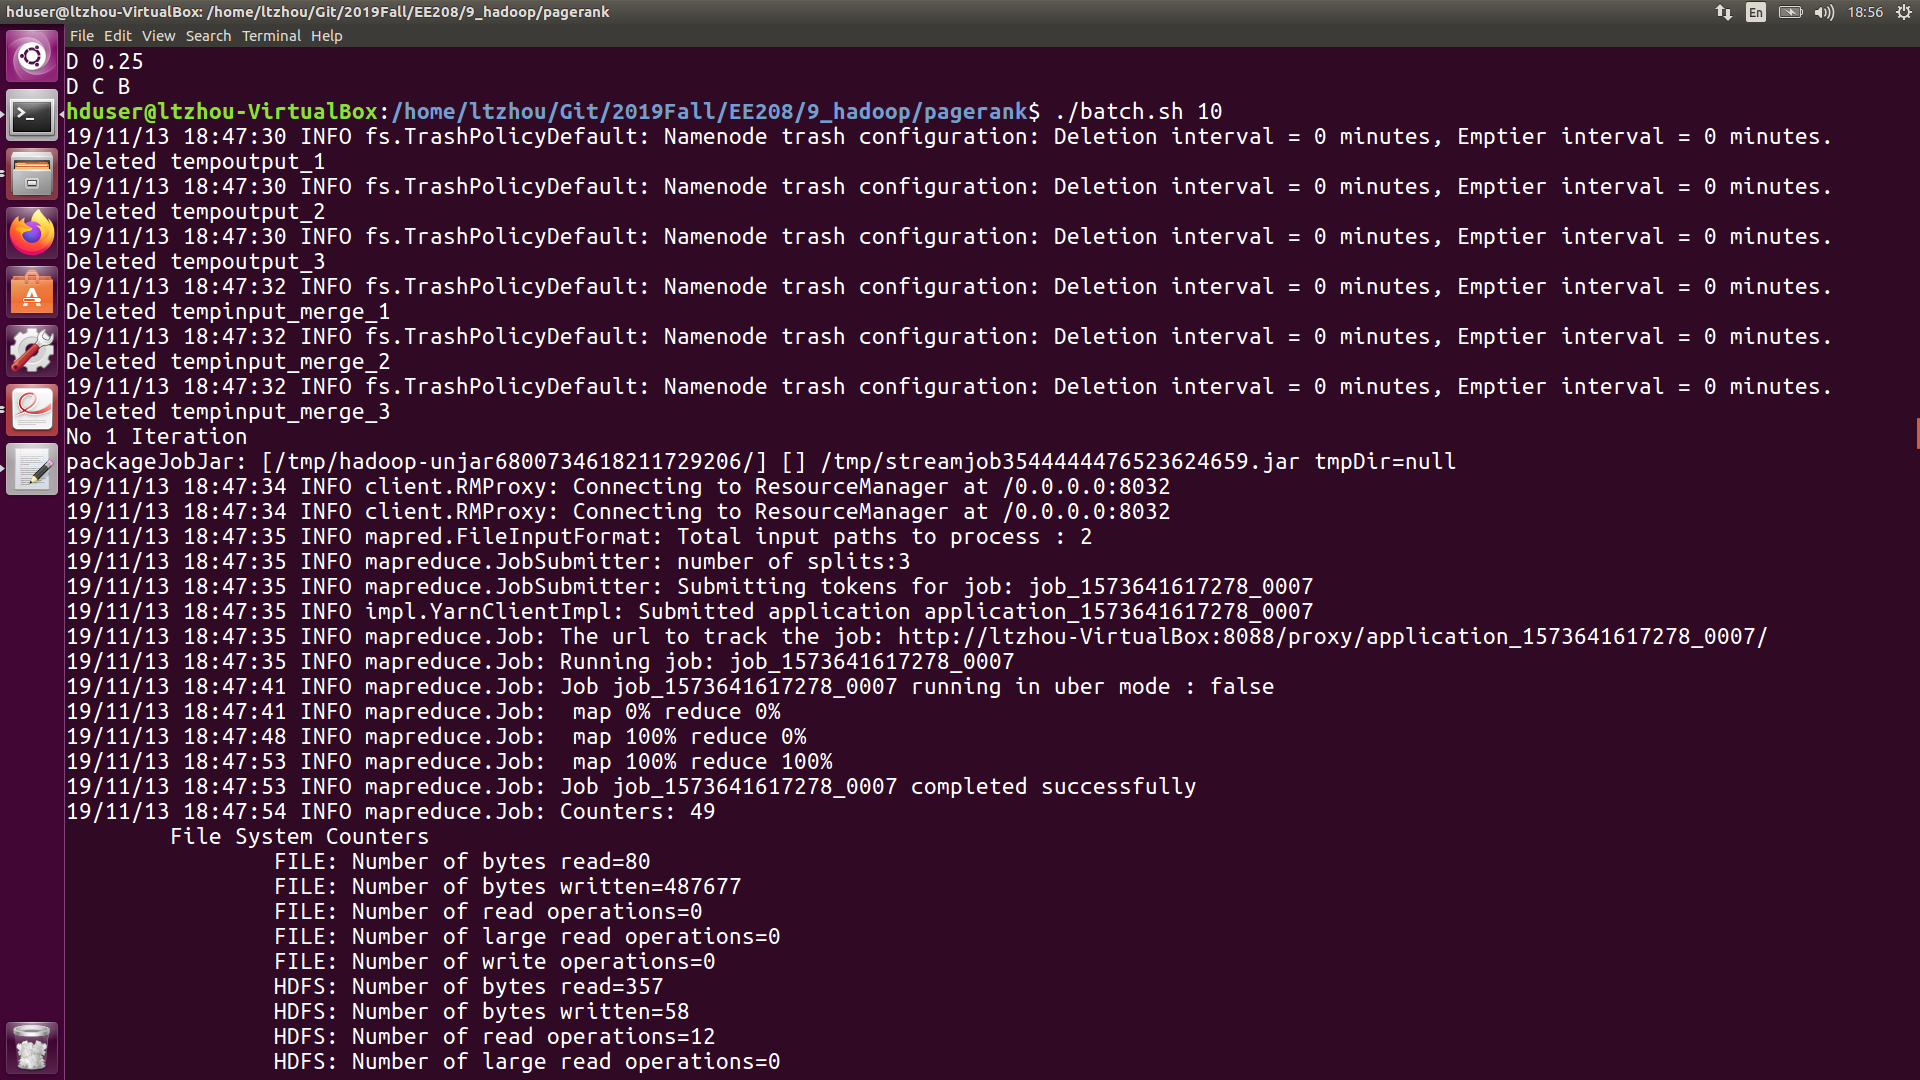
\includegraphics[width=7.5cm]{img/running_head.png}
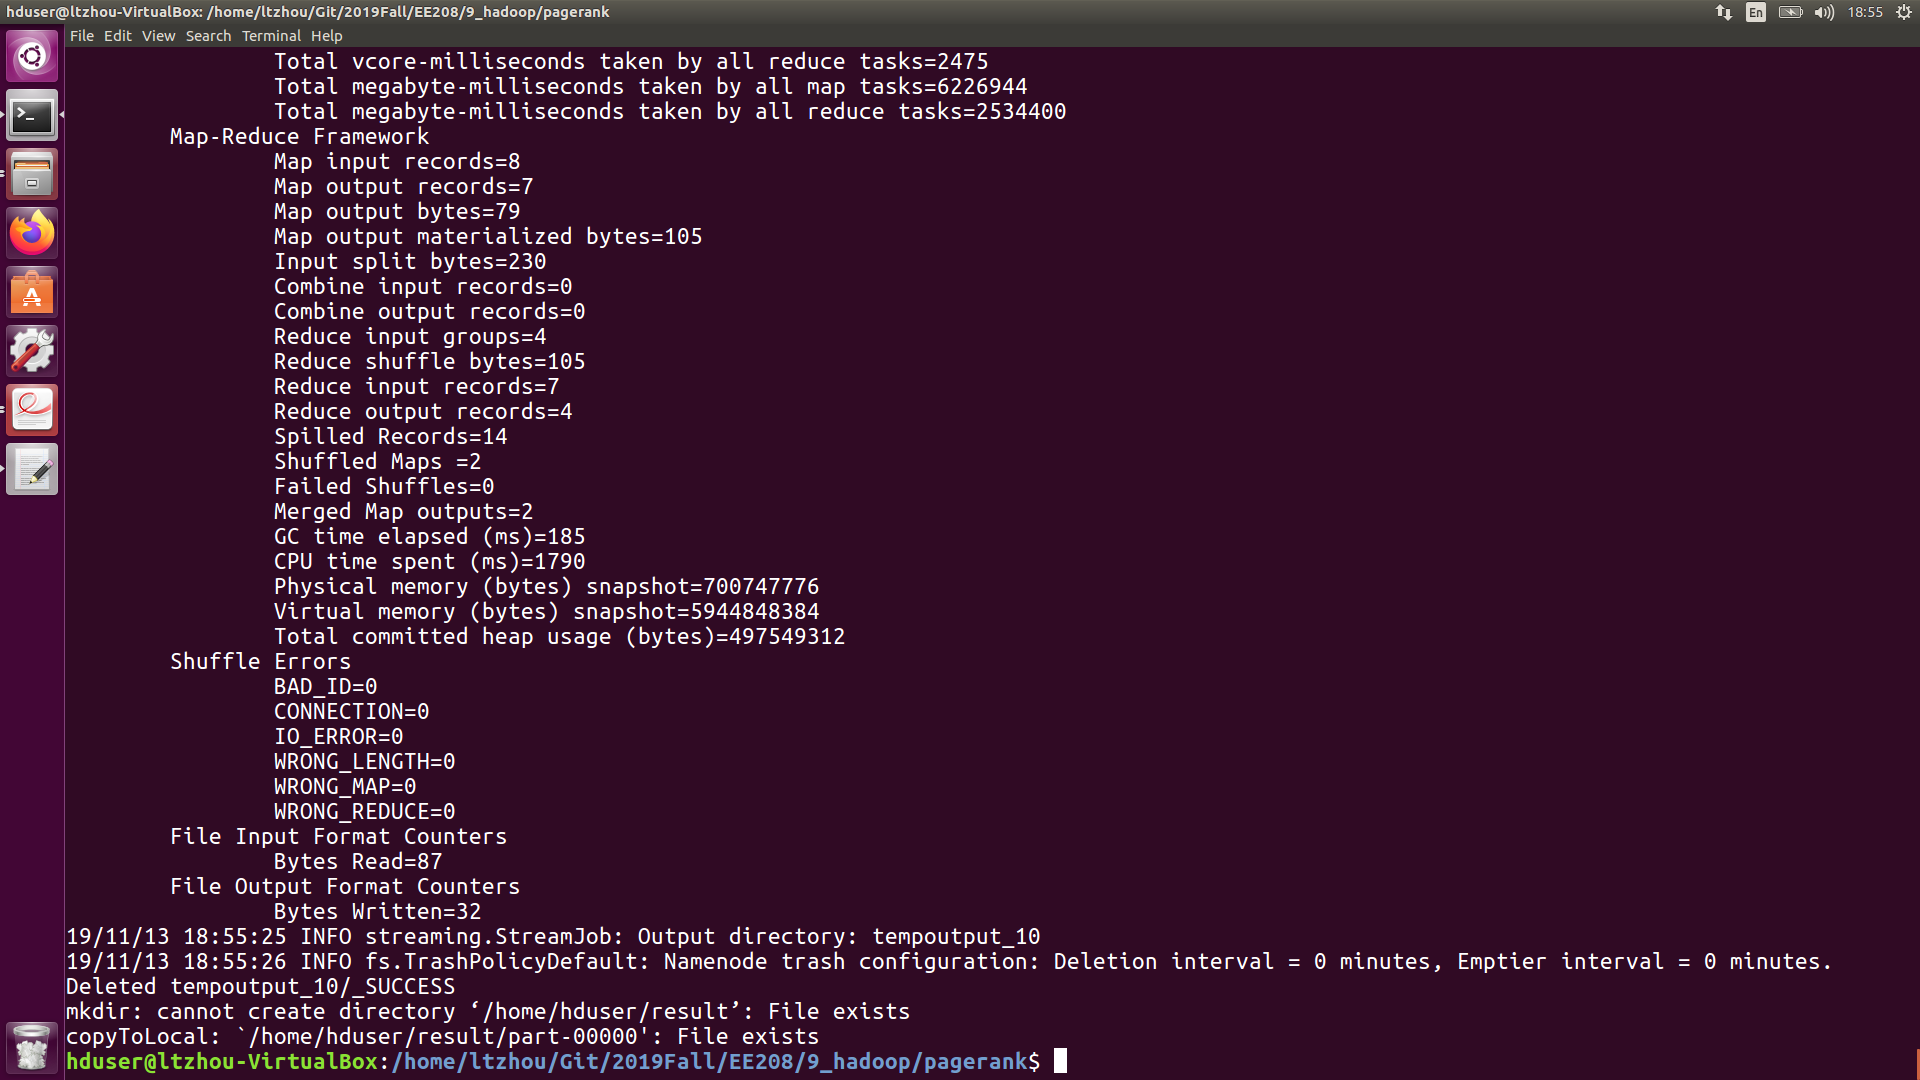
\includegraphics[width=7.5cm]{img/running_end.png}
\caption{PageRank计算程序运行示例}
\label{prrun}
\end{figure}


我们得到的不同迭代过程的输出如图\ref{prres}所示。

\begin{figure}[htbp]
\centering
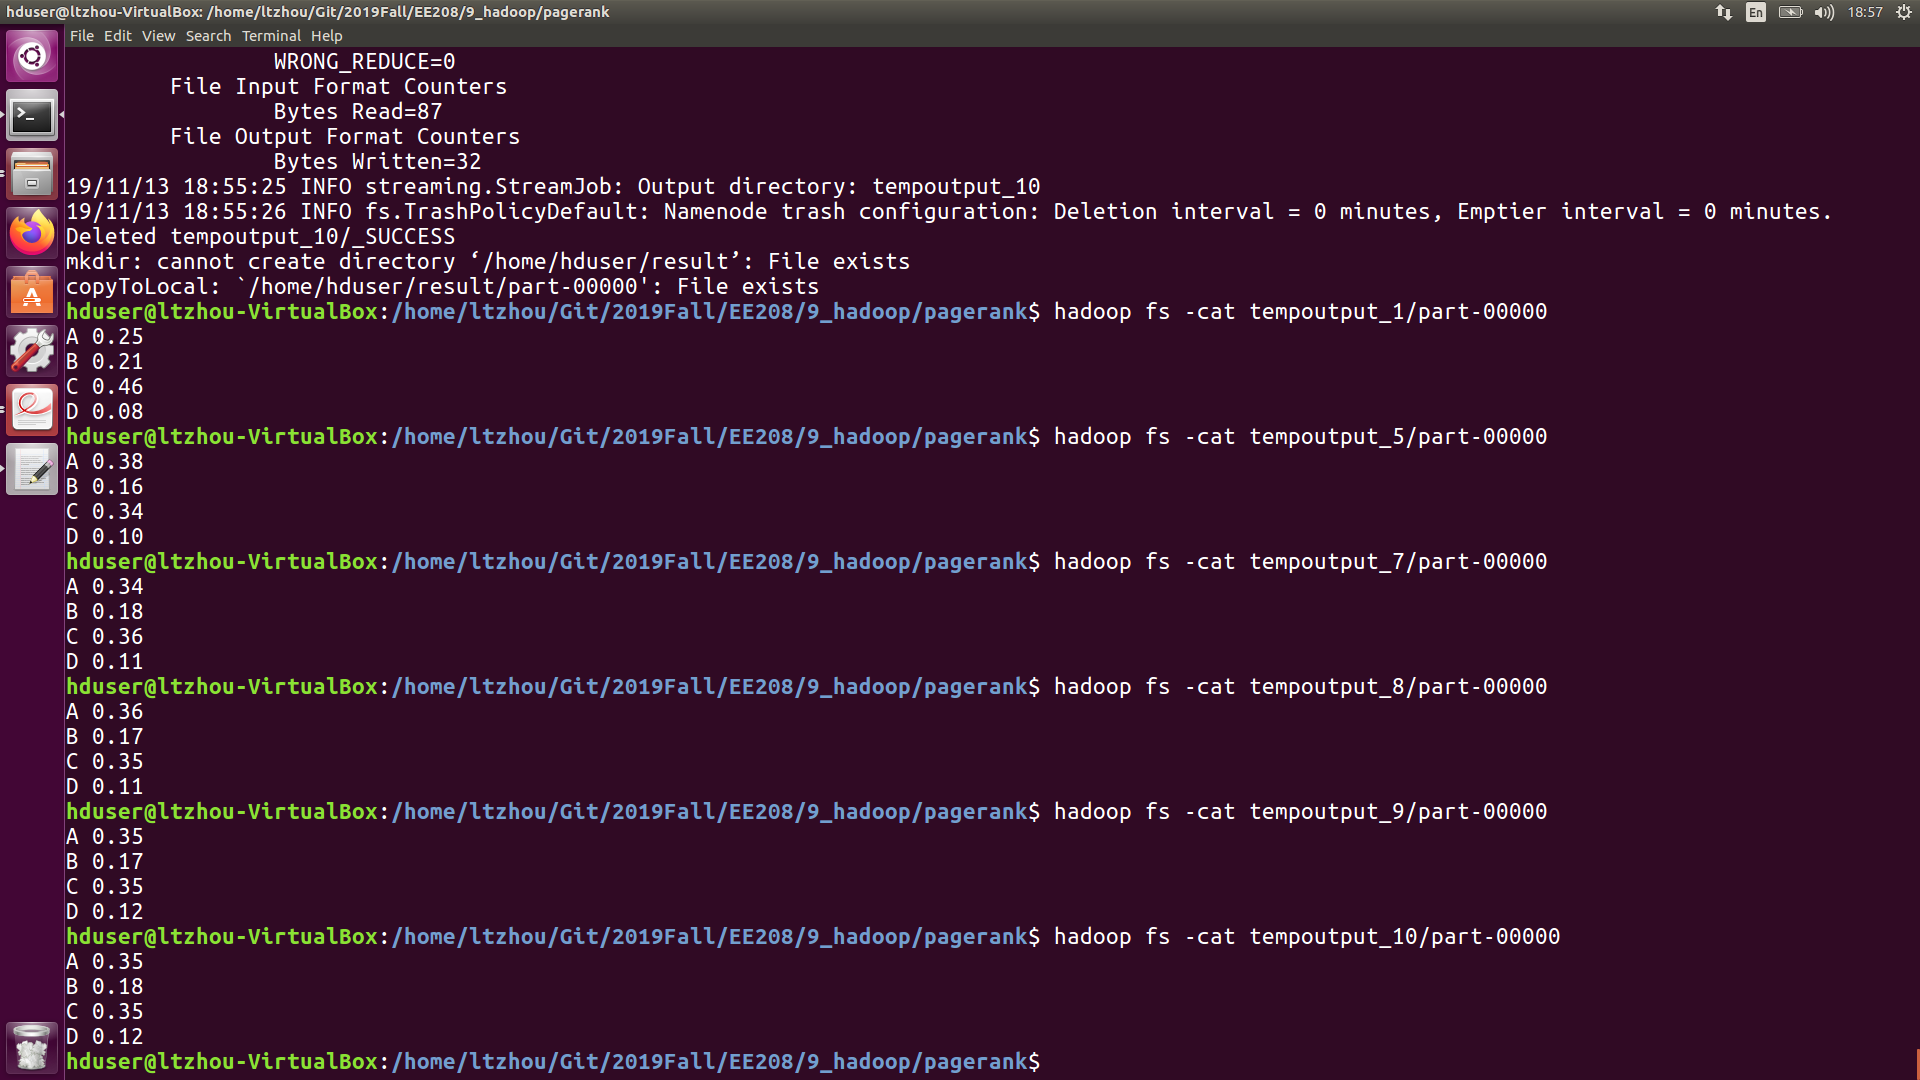
\includegraphics[width=14.5cm]{img/result.png}
\caption{PageRank计算结果示例}
\label{prres}
\end{figure}

每一次迭代的计算结果统计如下表所示。
\begin{center}
\begin{table}[]
\begin{tabular}{ccccc}
\hline
\textbf{Iteration} & \textbf{A} & \textbf{B} & \textbf{C} & \textbf{D} \\ \hline
1                  & 0.25       & 0.25       & 0.25       & 0.25       \\
2                  & 0.25       & 0.21       & 0.46       & 0.08       \\
3                  & 0.46       & 0.12       & 0.33       & 0.08       \\
4                  & 0.33       & 0.19       & 0.31       & 0.15       \\
5                  & 0.31       & 0.18       & 0.38       & 0.11       \\
6                  & 0.38       & 0.16       & 0.34       & 0.10       \\
7                  & 0.34       & 0.18       & 0.36       & 0.11       \\
8                  & 0.36       & 0.17       & 0.35       & 0.11       \\
9                  & 0.35       & 0.17       & 0.35       & 0.12       \\
10                 & 0.35       & 0.18       & 0.35       & 0.12       \\ \hline
\end{tabular}
\end{table}
\end{center}

可以观察到在6次迭代之后,PageRank数据已趋于稳定,数据上下浮动是因为浮点数的四舍五入造成的,这可以通过修改程序中的浮点数输出精度来提高。

\subsection{改进}
进一步,我们为迭代的过程加上系数0.85,在Map部分,只有0.85的PageRank会被分给它的子节点,剩余的PageRank则保留为本节点输出,修改后的Mapper代码如下所示。注意到这部分我们将输出的精度调整到四位小数,以得到更精确的PageRank。
\begin{python}
if (src != current_src):
   current_src = src
   current_rank = float(seg[1])*alpha                # 用于分配给出点的pagerank
   print '%s\t%.4f' % (src,float(seg[1])*(1-alpha))  # src节点的pagerank
\end{python}

改进后的实验中,我们使用了助教所给的实验数据,如下所示。

\begin{python}
# Graph Structure
src | dst      | Initial PageRank
-----------------------------------
 1  | 2 3 4    | 0.25
 2  | 3 4      | 0.25
 3  | 4        | 0.25
 4  | 2        | 0.25
\end{python}

得到的迭代结果可在result文件夹中找到。观察发现,在第十次迭代时,PageRank的计算值已接近收敛。

\section{实验总结}
\paragraph{概述}
本实验中,我们通过Hadoop的Map-Reduce框架,实现了分布式单词平均长度的计算和图结构PageRank的计算。

\paragraph{感想}
通过本次实验的学习,我体会到到了分布式运算在数据量较大时,能够带来的运算效率提升。分布式运算能够帮助我们更充分地利用、扩展现有的硬件资源。我也通过实验的尝试,进一步学习了MAP-REDUCE框架的思想,并学会了如何使用Bash实现Map-Reduce计算的迭代调用。

\paragraph{问题}
本实验中遇到的一个较大问题是在PageRank的计算中,常常会出现运行时报错。在Mapper、Reducer函数都能正常运行,第一次迭代也能输出正确结果的情况下,这种问题通常会发生在第二次迭代中,经过尝试发现问题出在浮点数的输出上。多次迭代后,浮点数往往是无限小数,因此若直接输出成字符串,会占用较长的空间,产生超时的问题。因此,我们在PageRank计算时,对中间值统一输出\textbf{有限精度位}的小数,解决了这一问题。在Map-Reduce过程中,由于分布式计算的框架与通常我们熟悉的单线程程序不同,常常会产生很多功能不能正常移植的问题,这时我们可以通过修改程序实现方法、引入更多中间过程、在程序中加入try-except机制等手段解决问题,实现分布式计算。

此外,本实验中也有一些可以在未来进一步改进的空间,如可以在统计词长时对特殊符号加以处理,使结果更准确。在PageRank的计算中,我们没有考虑成环的节点和边产生的“陷阱”对计算带来的影响,可以进一步加入带随机变量的计算来提升PageRank的表现。

\paragraph{创新}

首先,本实验中为两个实验都提供了运行的bash文件,做了良好的封装。其次,本实验在计算PageRank中,不同于通用的方法,我们将静态的图结构数据与不断迭代的PageRank数据分别保存、处理,有效地节约了每次输入输出的成本,减少了中间值的存储空间,相信会在数据量更大的情况下给出更好的运行效率。

\end{document}

